\documentclass[english,9pt]{extarticle}
\usepackage{babel}
\usepackage[dvipsnames]{xcolor}
\usepackage{hyperref}
\usepackage{geometry}
\usepackage{changepage}
\usepackage{graphicx}
\usepackage{array}
\usepackage{nth}
\usepackage[utf8]{inputenc}
\usepackage[T1]{fontenc}
\usepackage{csquotes}

%% Configure hyperref
\hypersetup{
	bookmarks=true,
	unicode=false,
	pdftoolbar=false,
	pdfmenubar=false,
	pdftitle={Curriculum Vitea - Duco van Amstel},
	pdfauthor={D. van Amstel},
	pdfcreator={D. van Amstel},
	pdfproducer={D. van Amstel},
	pdfkeywords={resume,curriculum vitae,cv},
	pdfnewwindow=true,
	colorlinks=true,
	allcolors=Blue,
	psdextra,
	unicode
}


%% Configure geometry
\geometry{
	top=0.5in,
	bottom=0.8in,
	margin=1in
}


%% Bibliography
\usepackage[
		citestyle=numeric,
		bibstyle=numeric-verb,
		sorting=none,
		defernumbers=true,
		backend=bibtexu,
		maxnames=8,
		minnames=4
	]{biblatex}

\addbibresource{../references/publications.bib}


%% Document
\begin{document}
%% Name
\begin{huge}
	\noindent Duco van Amstel
\end{huge}

\noindent\rule{0.8\textwidth}{2pt}
\begin{flushright}
\vspace{-2cm}
\raisebox{2cm}{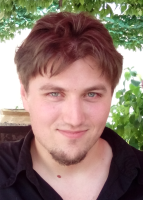
\includegraphics[width=80pt]{../references/cv_photo.png}}
\end{flushright}
\vspace{-4cm}


%% Contact details
\noindent
\begin{tabular}{b{0.3\textwidth}b{0.5\textwidth}}
	INRIA Antenne GIANT \newline
	MINATEC Campus \newline
	17 rue des Martyrs \newline
	38054 Grenoble Cedex 9 \newline
	FRANCE
	&
	Phone (mobile): +33 6 78 31 32 33 \newline
	Email: \href{mailto:duco.van.amstel@ens-lyon.org}{duco.van.amstel@ens-lyon.org} \newline
	Homepage: \url{www.helcaraxan.eu}
\end{tabular}

\noindent\rule{\textwidth}{1pt}


%% Education
\section*{Education}
\begin{adjustwidth}{1em}{}
	\begin{description}
		\item[{\makebox[1cm][l]{Ph.D}}] Computer Science \quad \textit{Université Grenoble Alpes},
			Grenoble, France \hfill 07 / 2016
		\item[{\makebox[1cm][l]{MSc.}}] Computer Science \quad \textit{\'Ecole Normale Supérieure de
			Lyon}, Lyon, France \hfill 06 / 2012 \\
			Passed with high honours (\textit{mention ``bien''})
		\item[{\makebox[1cm][l]{Bsc.}}] Computer Science \quad \textit{\'Ecole Normale Supérieure de
			Lyon}, Lyon, France \hfill 06 / 2010 \\
			Passed with high honours (\textit{mention ``bien''}) \\
			The \emph{\'Ecole Normale Supérieure} (ENS) is the most competitive French research school and
			university.
		\item[Preparatory Classes] \quad \textit{Louis le Grand}, Paris, France \hfill 2006 - 2009 \\
			Intensive program preparing for the competitive entry exams to French engineering schools. \\
			\emph{Louis le Grand} frequently ranks \nth{1} among the schools offering such a program.
	\end{description}
\end{adjustwidth}


\noindent\rule{\textwidth}{1pt}

%% Experience
\section*{Employment}
\begin{tabular}{p{0.14\textwidth}p{0.82\textwidth}}
	2013 -- 2016 & \textbf{R\&D engineer}, \textit{Kalray}, Grenoble, France \newline
		\href{www.kalray.eu}{Kalray} is a fabless semi-conductor company designing and supporting its
		own manycore processors: the MPPA family. This industry position accounted for half of my time
		as Ph.D student and allowed the implementation of my research work in an industrial environment.
		\newline
		\textit{Responsabilities: compiler engineering (GCC \& other tools), design and modelisation of
		a Network-on-Chip, developement and reporting for large scale collaborative projects.}
		\vspace{0.2cm} \\
	2013 -- 2016 & \textbf{Research assistant}, \textit{Inria}, Grenoble, France \newline
		Member of the \href{https://team.inria.fr/corse}{Corse} research team as part of my Ph.D.
		Development of heuristical tiling solvers, LLVM passes and the GraphUtilities library for convex
		partitioning and reachability queries.
		\newline \textit{Other assignments: system adminstrator \& IT purchases}
		\vspace{0.2cm} \\
	2013 -- 2016 & \textbf{Teaching assistant}, \textit{Université Grenoble Alpes / ENSIMAG},
		Grenoble, France \newline 
		Independent from my Ph.D work. Assisting in multiple courses.
		\vspace{0.2cm} \\
	2012 \newline March -- June & \textbf{MSc. intern}, \textit{Laboratoire d'Informatique de
		Grenoble}, Grenoble, France \newline
		Work on the Berkeley Open Infrastructure for Network Computing (BOINC).
		\vspace{0.2cm} \\
	2011 \newline March -- August & \textbf{MSc. intern}, \textit{Kalray}, Grenoble, France \newline
		R\&D for an architecture-specific bitslice implementation of the AES cryptographic protocol.
		\vspace{0.2cm} \\
	2010 \newline June -- July & \textbf{BSc. intern}, \textit{Inria}, Grenoble, France \newline
		Traffic flow modeling and prediction. Extension and simulation of a mathematical flow model.
		\vspace{0.2cm} \\
\end{tabular}


\noindent\rule{\textwidth}{1pt}

%% Research interests
\section*{Research interests}
\begin{adjustwidth}{1em}{}
	\begin{description}
		\item[Low-level \& target-specific optimizations] Tweaking code at instruction level, manually
			or with compilers, to achieve high performance and efficiency. Exploiting target specifics to
			reduce code size and execution time.
		\item[Micro-architecture] Studying interactions between a compiler toolchain and a target
			architecture. Improving the adequacy of the features offered by an architecture with respect
			to the needs of a compiler.
		\item[Graph algorithmics] Computation of graph characteristics, analysis of graph structures and
			other graph-based queries: reachability on DAGs, convex partitioning.
		\item[Heuristical approaches] Designing low complexity algorithms to compute potentially
			sub-optimal but efficient solutions to hard problems.
	\end{description}
\end{adjustwidth}


%% Publications
\section*{Publications}
\nocite{*}
\printbibliography[heading=subbibliography,title=Conferences \& workshops,type=inproceedings]
\printbibliography[heading=subbibliography,title=Thesis,type=thesis]
\printbibliography[heading=subbibliography,title=Patents,type=misc]


\noindent\rule{\textwidth}{1pt}

%% Software
\section*{Software}

\begin{adjustwidth}{1em}{}
	\begin{description}
		\item[GraphUtilities library] A library developed during my Ph.D for the manipulation and
			analysis of directed graphs. Its main features are fast multi-threaded reachability querying
			and convex partitioning. \\
			\textit{Available on GitHub at \url{https://github.com/Helcaraxan/GraphUtilities}.}
		\item[LLVM generalized tiling] Set of LLVM passes and tiling solvers which implement generalized
			register tiling as described in \cite{domagala:register_tiling:2016}. Work done together with
			co-author \L{}ukasz Domaga\l{}a. My contribution includes among other features the design and
			implementation of the heuristical tiling methods presented in
			\cite{domagala:dataflow_tiling:2016,vanamstel:data_locality:2016}. \\
			\textit{Not publicly available. Used by the CORSE research team @ Inria.}
		\item[Kalray toolchain] I made numerous contributions to the global software toolchain that
			supports the Kalray MPPA manycore chip. The main focus of these contributions were in the area
			of the specialized GCC back-end and other external code optimization tools. Also includes a
			simulator for the MPPA Network-on-Chip. \\
			\textit{Not publicly available. Part of Kalray's software products.}
	\end{description}
\end{adjustwidth}


\noindent\rule{\textwidth}{1pt}

%% References
\section*{References}
\begin{adjustwidth}{1em}{}
	\begin{description}
		\item[Benoît Dupont de Dinechin] -- CTO @ \textit{Kalray}, Grenoble, France \\
			Kalray S.A \\
			445 rue Lavoisier / 38330 Montbonnot \\
			FRANCE \\
			\href{mailto:benoit.dinechin@kalray.eu}{benoit.dinechin@kalray.eu}
		\item[Fabrice Rastello] -- Research team leader @ \textit{Inria}, Grenoble, France \\
			INRIA Antenne GIANT / MINATEC Campus \\
			17 rue des Martyrs / 38054 Grenoble Cedex 9 \\
			FRANCE \\
			\href{mailto:fabrice.rastello@inria.fr}{fabrice.rastello@inria.fr}
	\end{description}
\end{adjustwidth}

\clearpage


%% Reviews
\section*{Reviewing}
\begin{tabular}{p{0.15\textwidth}p{0.81\textwidth}}
	External reviewer & DATE'16, CGO'15, CGO'14
\end{tabular}

\noindent\rule{\textwidth}{1pt}

%% Awards & grants
\section*{Awards \& grants}
\begin{tabular}{p{0.1\textwidth}p{0.86\textwidth}}
	2016 &
	ACM Student Research Competition @ CGO '16 -- \nth{2} place
	\\
	2013 &
	Selected for a 3-year CIFRE Ph.D funding
	\vspace{0.2cm} \\
\end{tabular}


\noindent\rule{\textwidth}{1pt}

%% Teaching experiences 
\section*{Teaching experiences}
\begin{adjustwidth}{1em}{}
	\begin{description}
		\item[Introduction to Algorithmics and C] \quad Undergraduate - \nth{1} semester \hfill Fall
			2014 \\
			Introductory course for first-year CS students. Core concepts of computer programming and
			algorithmics. \\
			\textit{Responsible for teaching, practice sessions and grading for a single student group
			($\sim$40 students)}
		\item[Logical Circuitry \& Processor Architecture] \quad Undergraduate - \nth{5} semester \hfill
			Fall 2013 -- 2015\\
			Third-year course teaching the basics of circuitry design to software engineering students.
			The semester finishes with the specification of a small CISC processor and its simulation. \\
			\textit{Responsible for practice sessions and part of grading ($\sim$40 students)}
		\item[Advanced Algorithmics] \quad Undergraduate - \nth{6} semester \hfill Spring 2013 -- 2015
			\\
			First-year course at the ENSIMAG engineering school ($\sim$\nth{3} year of college). Various
			data structures and their algorithmic properties. \\
			\textit{Responsible for grading of small student projects ($\sim$140 students)}
		\item[Team-based end-of-year projects] \quad Undergraduate - \nth{6} semester \hfill Spring 2013
			-- 2016 \\
			First-year course at the ENSIMAG engineering school ($\sim$\nth{3} year of college). Full-time
			2-week team coding projects. Various subjects: graphical interface library, MIPS simulator,
			\dots \\
			\textit{Member of a 10-person staff advising and grading ($\sim$300 students)}
	\end{description}
\end{adjustwidth}


\noindent\rule{\textwidth}{1pt}

%% Languages
\section*{Languages}
\begin{adjustwidth}{1em}{}
	English - \textit{fluent}, French - \textit{fluent}, Dutch - \textit{mothertongue}, German -
	\textit{working knowledge}, Swedish - \textit{beginner}
\end{adjustwidth}

\end{document}
